\documentclass{article}

\usepackage{graphicx}
\usepackage{multirow}
\usepackage{amsmath}
\title{Note: Linear Regression Model}
\author{Sun Zhao}

\begin{document}
\maketitle
\newpage

\section{Model Representation}
Remind that regression algorithms are tying to infer a function predicting continuous values when given training samples. Let's first focus on the notation of the training samples. Regarding to Table1, training samples are represented by a vector of \textbf{x} and a vector of \textbf{y} with identical length of m and each sample becomes a pair of ($x^{(i)}$, $y^{(i)}$). The inferred function h(which means hypothesis) is shown as below:\\

\begin{equation}\label{hypothesis_function}
  h_\Theta(x)=\Theta_0 + \Theta_1x
\end{equation}
For simplicity, (\ref{hypothesis_function}) consists of only one variable, thus we call this linear regression as univariate linear regression.

\section{Cost Function}
$\Theta_0$ and $\Theta_1$ are the two arguments of hypothesis function, so the idea here is to choose optimal values of $\Theta_0$ and $\Theta_1$. Intuitively, the optimal h should minimize average the error distance between the predict values of each $x^(i)$ and $y^(i)$. Then we can define the cost function as below:
\begin{equation}\label{cost_function}
J(\Theta_0, \Theta_1) = \frac{1}{2m} \sum_{i=1}^{m} (h_\Theta({x^{(i)}})-y^{(i)})^2
\end{equation}
Obviously, the object function is defined as:
\begin{equation}\label{object_function}
\underset{\Theta_0, \Theta_1}{minimize} \frac{1}{2m} \sum_{1}^{m} (h_\Theta({x^{(i)}})-y^{(i)})^2
\end{equation}
Using the cost function, we can easily calculate the cost value of any hypothesis functions. For example, Fig. \ref{examples_hypothesis_plot} shows three samples(cross pointers) and a hypothesis function $h(x)=0.5x$. The cost value of it is calculated as:
\begin{equation}\label{cost_function_example}
J(0.5)=\frac{1}{2 \times 3}[(0.5-1)^2 + (1-2)^2 + (1.5-3)^2]=\frac {3.5}{6}
\end{equation}
\begin{figure}[ht]
  \centering
  % Requires \usepackage{graphicx}
  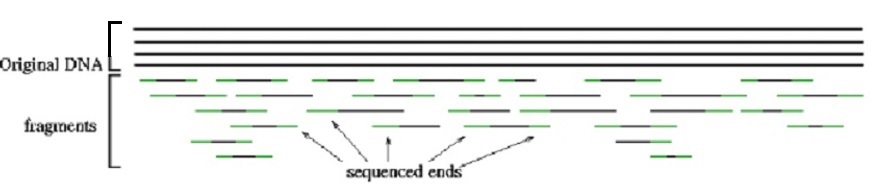
\includegraphics[width=5cm]{Figure1.jpg}\\
  \caption{}\label{examples_hypothesis_plot}
\end{figure}
\section{Gradient Descent}
Now we turn to the calculation methods of the objection function. Suppose we have a training set as shown in Fig. \ref{training_dataset}. We can enumerate all the possible values of $\Theta_0$ and $\Theta_1$ and calculate the corresponding cost $J(\Theta_0, \Theta_1$) and show them in a 3D space like Fig \ref{3D_cost_function_plot}. In Fig. \ref{3D_cost_function_plot}, if we start from a random pointer$(\Theta_0, \Theta_1, J(\Theta_0, \Theta_1))$, we can iteratively migrate a small step through the negative direction of the gradient direction of this point and hopefully, we will converge to the lowest point of the surface.
\begin{figure}[ht]
  \centering
  % Requires \usepackage{graphicx}
  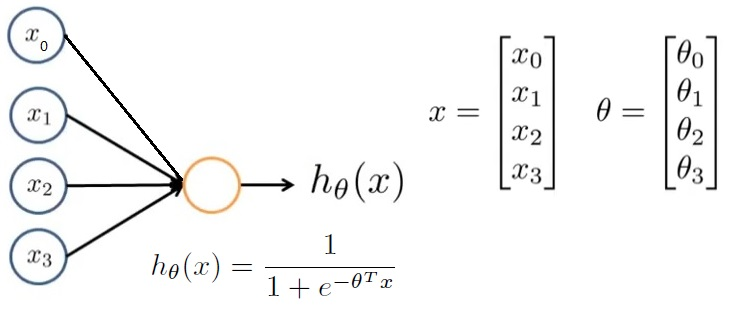
\includegraphics[width=5cm]{Figure2.jpg}\\
  \caption{}\label{3D_cost_function_plot}
\end{figure}
\begin{figure}[ht]
  \centering
  % Requires \usepackage{graphicx}
  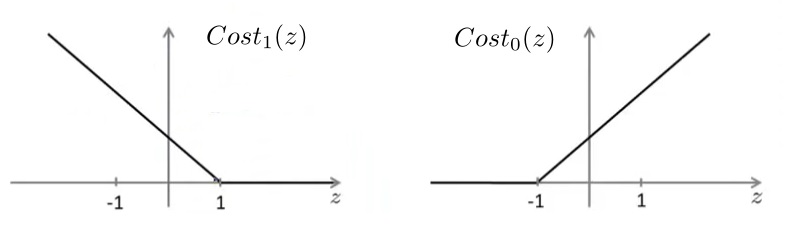
\includegraphics[width=5cm]{Figure3.jpg}\\
  \caption{}\label{training_dataset}
\end{figure}
\newline Formally, we describe gradient descent algorithm as following:\\
Algorithm1:\\
$\Theta_0 = 0;$\\
$\Theta_1 = 0;$\\
repeat until convergence\{\\
$\Theta_j = \Theta_j - \alpha\frac{\partial}{\partial \theta_j}J(\theta_0, \theta_1) for(j = 0 and j = 1)$\\
\}\\
Issue1: $\alpha$ is called the learning rate. It is a pre-choose value, and if it is too small, the convergence process will be much slow, and otherwise it is too large, it can not converge and possibly diverge. As the algorithm approach a local minimum, gradient descent will automatically take smaller steps. So, no need to decrease $\alpha$ over time.\\
Issue2: The update process should be a simultaneous update which should be performed as:\\
$temp0=\Theta_0 - \alpha\frac{\partial}{\partial \theta_0}J(\theta_0, \theta_1)$\\
$temp1=\Theta_1 - \alpha\frac{\partial}{\partial \theta_1}J(\theta_0, \theta_1)$\\
$\theta_0 = temp0$\\
$\theta_1 = temp1$\\
If we do not take a simultaneous update, the output of gradient descent algorithm is not defined.\\
Issue3: Gradient Descent algorithm starts from a random point, so the output is a local optima instead of global optima. However, if the object function is a convex function, it is guaranteed that gradient descent algorithm will reach the global optima.\\
Get back to the linear regression problem, we use gradient descent to solve the problem of (\ref{object_function}). If we apply (\ref{hypothesis_function}) to algorithm1 and calculate the differential result, we will get:\\
repeat until convergence \{\\
$\theta_0=\theta_0 - \alpha \frac{1}{m} \sum_{i=1}^{m}(h_\theta(x^{(i)})-y^{(i)})$\\
$\theta_1=\theta_1 - \alpha \frac{1}{m} \sum_{i=1}^{m}(h_\theta(x^{(i)})-y^{(i)}) \cdot x^{(i)}$\\
\}\\
Note that we use all the samples to update the arguments in each step, so we called it "batch" gradient descent. Until now, linear regression problem is successfully solved by "batch" gradient descent.

\section{Summary}
Univariate linear regression model is represented as (\ref{hypothesis_function}), and its cost function and objection function are shown as (\ref{cost_function}) and (\ref{object_function}) separately. Apply object function with gradient descent algorithm will solve linear regression problem.

\end{document}
